% --------------------------------------------------------------------------- %
% Poster for the ECCS 2011 Conference about Elementary Dynamic Networks.      %
% --------------------------------------------------------------------------- %
% Created with Brian Amberg's LaTeX Poster Template. Please refer for the     %
% attached README.md file for the details how to compile with `pdflatex`.     %
% --------------------------------------------------------------------------- %
% $LastChangedDate:: 2011-09-11 10:57:12 +0200 (V, 11 szept. 2011)          $ %
% $LastChangedRevision:: 128                                                $ %
% $LastChangedBy:: rlegendi                                                 $ %
% $Id:: poster.tex 128 2011-09-11 08:57:12Z rlegendi                        $ %
% --------------------------------------------------------------------------- %
\documentclass[a0paper,portrait]{baposter}

\usepackage{relsize}		% For \smaller
\usepackage{url}			% For \url
\usepackage{epstopdf}	% Included EPS files automatically converted to PDF to include with pdflatex
\usepackage{cite}
\usepackage{xcolor}

\usepackage{setspace}
\usepackage{amsmath}
\usepackage{mdwlist}
\usepackage{graphicx,stfloats}
\usepackage{booktabs}

\usepackage{siunitx}
\sisetup{per=slash, load=abbr}

\usepackage{calc}
\usepackage{array}
\usepackage{caption}
\usepackage{rotating}
\usepackage{url}
\usepackage{pgf,tikz}
\usepackage{pgfplots, pgfplotstable}
\usetikzlibrary{snakes,arrows,shapes}

\pgfplotsset{compat=newest}

%%% Global Settings %%%%%%%%%%%%%%%%%%%%%%%%%%%%%%%%%%%%%%%%%%%%%%%%%%%%%%%%%%%

\graphicspath{{pix/},{plots/}}	% Root directory of the pictures 
\tracingstats=2			% Enabled LaTeX logging with conditionals

%%% Color Definitions %%%%%%%%%%%%%%%%%%%%%%%%%%%%%%%%%%%%%%%%%%%%%%%%%%%%%%%%%

\definecolor{bordercol}{RGB}{255,255,255}
\definecolor{headercol1}{RGB}{186,215,230}
\definecolor{headercol2}{RGB}{186,215,230}
\definecolor{headerfontcol}{RGB}{0,0,0}
\definecolor{boxcolor}{RGB}{255,255,255}
%\definecolor{boxcolor}{RGB}{186,215,230}

%%%%%%%%%%%%%%%%%%%%%%%%%%%%%%%%%%%%%%%%%%%%%%%%%%%%%%%%%%%%%%%%%%%%%%%%%%%%%%%%
%%% Utility functions %%%%%%%%%%%%%%%%%%%%%%%%%%%%%%%%%%%%%%%%%%%%%%%%%%%%%%%%%%

%%% Save space in lists. Use this after the opening of the list %%%%%%%%%%%%%%%%
\newcommand{\compresslist}{
	\setlength{\itemsep}{1pt}
	\setlength{\parskip}{0pt}
	\setlength{\parsep}{0pt}
}

%%%%%%%%%%%%%%%%%%%%%%%%%%%%%%%%%%%%%%%%%%%%%%%%%%%%%%%%%%%%%%%%%%%%%%%%%%%%%%%
%%% Document Start %%%%%%%%%%%%%%%%%%%%%%%%%%%%%%%%%%%%%%%%%%%%%%%%%%%%%%%%%%%%
%%%%%%%%%%%%%%%%%%%%%%%%%%%%%%%%%%%%%%%%%%%%%%%%%%%%%%%%%%%%%%%%%%%%%%%%%%%%%%%

\begin{document}
\typeout{Poster rendering started}

%%% Setting Background Image %%%%%%%%%%%%%%%%%%%%%%%%%%%%%%%%%%%%%%%%%%%%%%%%%%
\background{
	\begin{tikzpicture}[remember picture,overlay]%
	\draw (current page.north west)+(-2em,2em) node[anchor=north west]
	{};
	%{\includegraphics[height=1.1\textheight]{background}};
	\end{tikzpicture}
}

%%% General Poster Settings %%%%%%%%%%%%%%%%%%%%%%%%%%%%%%%%%%%%%%%%%%%%%%%%%%%
%%%%%% Eye Catcher, Title, Authors and University Images %%%%%%%%%%%%%%%%%%%%%%
\begin{poster}{
	grid=false,
	% Option is left on true though the eyecatcher is not used. The reason is
	% that we have a bit nicer looking title and author formatting in the headercol
	% this way
	%eyecatcher=false, 
	borderColor=bordercol,
	headerColorOne=headercol1,
	headerColorTwo=headercol2,
	headerFontColor=headerfontcol,
	% Only simple background color used, no shading, so boxColorTwo isn't necessary
	boxColorOne=boxcolor,
	headershape=roundedright,
	headerfont=\large\sf\bf,
	textborder=rectangle,
	background=user,
	headerborder=open,
  boxshade=plain
}
%%% Logo %%%%%%%%%%%%%%%%%%%%%%%%%%%%%%%%%%%%%%%%%%%%%%%%%%%%%%%%%%%%%%%%%%%%%%
{
	% The logos are compressed a bit into a simple box to make them smaller on the result
	% (Wasn't able to find any bigger of them.)
	\setlength\fboxsep{0pt}
	\setlength\fboxrule{0pt}
	\fbox{
		\begin{minipage}{15em}
			\includegraphics[width=15em]{logo}
		\end{minipage}
	}
	
}
%%%% Eye Cacther %%%%%%%%%%%%%%%%%%%%%%%%%%%%%%%%%%%%%%%%%%%%%%%%%%%%%%%%%%%%%%%
%{
%	Eye Catcher, empty if option eyecatcher=false - unused
%}
%%% Title %%%%%%%%%%%%%%%%%%%%%%%%%%%%%%%%%%%%%%%%%%%%%%%%%%%%%%%%%%%%%%%%%%%%%
{\huge\sf\bf
Accelerator Design at High Level of \\ Programming Abstraction 
%Hardware Acceleration Without The Use Of ~RTL
}
%%% Authors %%%%%%%%%%%%%%%%%%%%%%%%%%%%%%%%%%%%%%%%%%%%%%%%%%%%%%%%%%%%%%%%%%%
{
	\vspace{0.3em} Prashant Ravi, Abhishek Kumar Jain, Suhaib A. Fahmy, Douglas L. Maskell\\
	{\smaller prashant014@ntu.edu.sg, abhishek013@ntu.edu.sg, s.fahmy@warwick.ac.uk, asdouglas@ntu.edu.sg}
}



\headerbox{Background and Motivation}{name=problem,column=0,row=0}{
Accelerator Design Productivity Issues:
%Major issues in mainstream adoption of FPGAs:
\begin{itemize}\itemsep1pt \parskip0pt
\item Difficulty of accelerator design at low level
\item Complex Host-Accelerator interfacing 
\item Lack of software like abstractions 
\item Long compilation times (Place and route)
\end{itemize}
One solution: High Level Synthesis (HLS)
\begin{itemize}\itemsep1pt \parskip0pt
\item Accelerator design in a high level language
\item Automated host-accelerator interfacing
\item RTL generation from C/C++/OpenCL
\item Benefits of software like abstractions 
\item SDSoC, \textbf{AOCL}, SDAccel
\item Long compilation time still an issue
\end{itemize}
Coarse-Grained FPGA Overlays:
\begin{itemize}\itemsep1pt \parskip0pt
\item Fast compilation and development cycles	
\item Easy to use even by novice programmers
\item Access of FPGA for software developers	
\item \textbf{MXP}, GRVI-Phalanx, DeCO, DySER
\end{itemize}
}



\headerbox{Contributions}{name=scgra,column=0,below=problem}{
\begin{itemize}\itemsep1pt \parskip0pt
	\item Analysis of Overlay architectures like Vectorblox MXP and Altera OpenCL SDK as alternatives to pure RTL design flow. Highlighting the ease of use and fast learning curves of these methods.
	\item Benchmarking and comparison of timing performance as well as operations per cycle for the Vectorblox MXP processor and the Altera OpenCL Implementation with arm CPU implementation.
\end{itemize}


}



\headerbox{Observations}{name=analysis, column=0,below=scgra}{
The Vectorblox MXP soft vector processor:
\begin{itemize}\itemsep1pt \parskip0pt
	\item Extremely short learning curve
	\item Easy to use MXP C/C++ APIs 
%	\item Full control of DMA and execution to programmer
	\item Compilation and debugging time equal to that of traditional C/C++ debugging
\end{itemize}
The Altera OpenCL SDK:
\begin{itemize}\itemsep1pt \parskip0pt
	\item Minimal modification of traditional OpenCL code required
	\item Kernel optimizations like vectorization, hardware replication for parallelism
%	\item FPGA reconfiguration at runtime with new kernel
	\item Host code portability across all devices
\end{itemize}	
	

}



\headerbox{Conclusions and Future Work}{name=conclusion,column=0,below=analysis,above=bottom}{
\begin{itemize}\itemsep1pt \parskip0pt
	\item More popularity of overlays and high level synthesis tools
	\item Place and route effeciency improvements in OpenCL to hardware
	\item Overall generated hardware effeciency improvment
	\item More awareness in the software world and amongst software developers
\end{itemize}
} 



\headerbox{The Vectorblox MXP Processor}{name=designmethod,column=1,row=0}{ 
\begin{itemize}\itemsep1pt \parskip0pt
	\item Accelerating Bare metal C/C++ applications on Zynq using MXP
	\item Easy to use software APIs for embedded vector processing
	\item 16 vector lanes each containing an ALU
	\item Good for integer operations, lacks floating point
\end{itemize}
%\vspace{-0.2em}
\setlength\fboxsep{0pt}
\setlength\fboxrule{0pt}
\begin{center}
\fcolorbox{white}{white!100}{
    \fbox{
        \begin{minipage}{19.4em}
        \begin{center}   
        \includegraphics[width=15em]{mxpflow}   	
		\includegraphics[width=15em]{vectorlane}
        \end{center}       	
        \end{minipage}
    }
}
\end{center}
}



\headerbox{DE0-NANO-SoC with OpenCL}{name=functionalunit,column=2,row=0}{
\begin{itemize}\itemsep1pt \parskip0pt
	\item Creation of a semi-customized pipelined datapath using OpenCL Kernels. 
	\item Full control of hardware replication at the kernel level with loop unrolling.
	\item Functional C emulator for functional verification wihout generating hardware.
	\item Special AOCL optimizations for floating point to reduce area.
	\item Dedicated AOCL memory channels for data transfer to and from accelerator.	
\end{itemize}	
	%\vspace{-0.2em}
	\setlength\fboxsep{0pt}
	\setlength\fboxrule{0pt}
	\begin{center}
		\fcolorbox{white}{white!100}{
			\fbox{
				\begin{minipage}{19.4em}
					\begin{center}   
						\includegraphics[width=10em]{aoclflow}
					\end{center}       	
				\end{minipage}
			}
		}
	\end{center}	
}

\headerbox{Quick Easy Mapping of Compute Kernels}{name=setup,span=2,column=1,below=functionalunit}{
\begin{center}   
	\includegraphics[width=35em]{codesnip}
\end{center}
}

\headerbox{Experimental Evaluation(12-Tap FIR)}{name=experiment1,span=2,column=1,below=setup,above=bottom}{	

\setlength\fboxrule{0pt}
\begin{center}
	\fcolorbox{white}{white!100}{
		\fbox{



	\begin{minipage}{13em}
	\begin{center}      	
		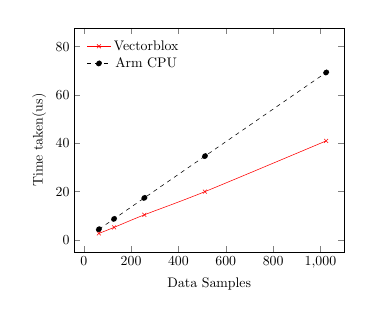
\begin{tikzpicture}[scale=0.5]
		\begin{axis}[
		xlabel=Data Samples,
		enlarge y limits = true,
		ylabel=Time taken(us),
		ymax = 80,
		xmax = 1100,
		legend pos=north west,
		legend style={draw=none}
		]
		\addplot [smooth,mark=x,red] plot coordinates {
			(64,     2.7)
			(128,    5.2)
			(256,    10.4)
			(512,    20)
			(1024,   41)			
		};
		\addplot [smooth,mark=*,dashed] plot coordinates {
			(64,     4.43)
			(128,    8.71)
			(256,    17.4)
			(512,    34.69)
			(1024,   69.30)
			
		};
		\legend{Vectorblox\\Arm CPU\\}
		\end{axis}
		\end{tikzpicture}
	\end{center}  
	\tiny  
	Vectorblox C API Implementation in Comparison with naive C Implementation on ARM CPU.
	\end{minipage}

	\hspace{1em}
	\begin{minipage}{13em}
	\begin{center}      				
	 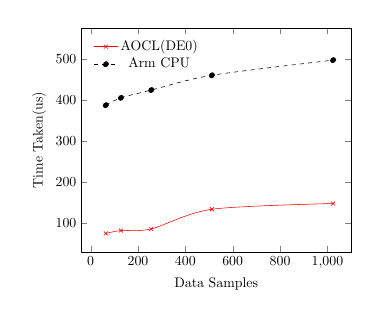
\begin{tikzpicture}[scale=0.5]
	 \begin{axis}[
	 xlabel=Data Samples,
	 ylabel=Time Taken(us),
	 enlarge y limits = true,
	 ymax = 530,
	 xmax = 1100,
	 legend pos=north west,
	 legend style={draw=none}
	 ]
	 \addplot [smooth,mark=x,red] plot coordinates {
			(64,     74)
			(128,    81)
			(256,    85)
			(512,    133)
			(1024,   147)			
		};
		\addplot [smooth,mark=*,dashed] plot coordinates {
			(64,     387)
			(128,    405)
			(256,    424)
			(512,    460)
			(1024,   497)
			
		};
	 \legend{AOCL(DE0)\\Arm CPU\\}
	 \end{axis}
	 \end{tikzpicture}
	\end{center}
	\tiny 
	OpenCL Implementation Timing Comparison between ARM CPU and AOCL FPGA Implementation.   					
	\end{minipage}
					
		}
	}
\end{center}



\vspace{-2em}

\setlength\fboxrule{0pt}
\begin{center}
	\fcolorbox{white}{white!100}{
		\fbox{



	\begin{minipage}{13em}
	\begin{center}      	
		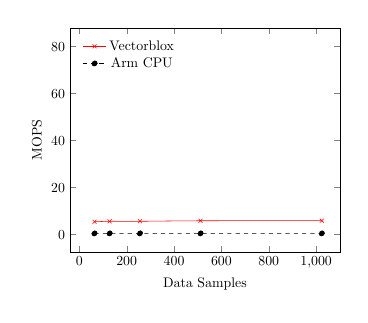
\begin{tikzpicture}[scale=0.5]
		\begin{axis}[
		xlabel=Data Samples,
		enlarge y limits = true,
		ylabel=MOPS,
		ymax = 80,
		xmax = 1100,
		legend pos=north west,
		legend style={draw=none}
		]
		%vbx
		\addplot [smooth,mark=x,red] plot coordinates {
			(64,     5.451)
			(128,    5.661)
			(256,    5.661)
			(512,    5.888)
			(1024,   5.924)			
		};
		%arm
		\addplot [smooth,mark=*,dashed] plot coordinates {
			(64,     0.497)
			(128,    0.506)
			(256,    0.507)
			(512,    0.508)
			(1024,   0.509)
			
		};
		\legend{Vectorblox\\Arm CPU\\}
		\end{axis}
		\end{tikzpicture}
	\end{center}  
	\tiny  
	Vectorblox C API Implementation in Comparison with naive C Implementation on ARM CPU.
	\end{minipage}

	\hspace{1em}
	\begin{minipage}{13em}
	\begin{center}      				
	 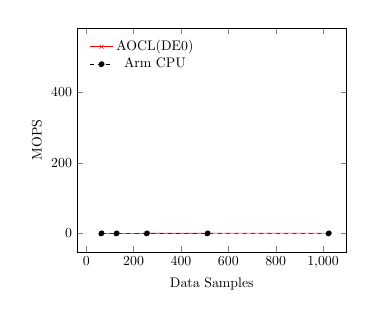
\begin{tikzpicture}[scale=0.5]
	 \begin{axis}[
	 xlabel=Data Samples,
	 ylabel=MOPS,
	 enlarge y limits = true,
	 ymax = 530,
	 xmax = 1100,
	 legend pos=north west,
	 legend style={draw=none}
	 ]
	 \addplot [smooth,mark=x,red] plot coordinates {
			(64,     0.1301)
			(128,    0.2378)
			(256,    0.4532)
			(512,    0.5793)
			(1024,   1.0483)			
		};
		\addplot [smooth,mark=*,dashed] plot coordinates {
			(64,     0.00570)
			(128,    0.01089)
			(256,    0.0208)
			(512,    0.0383)
			(1024,   0.0710)
			
		};
	 \legend{AOCL(DE0)\\Arm CPU\\}
	 \end{axis}
	 \end{tikzpicture}
	\end{center}
	\tiny 
	OpenCL Implementation Timing Comparison between ARM CPU and AOCL FPGA Implementation.   					
	\end{minipage}
					
		}
	}
\end{center}



\vspace{-2em}	

%\begin{itemize}\itemsep1pt \parskip0pt
%	\item The MXP gave a \textbf{1.6x Operations Per Cycle} increase over ARM and a \textbf{1.5x Speedup}.
%	\item The AOCL implementation gave \textbf{3.3x Operations per Cycle} increase over ARM with a \textbf{4x Speedup}.
%\end{itemize}	

}
\end{poster}
\end{document}
